\section{Results and Discussion}\label{sec:results}
While the \ac{db2} contains \var{entries_db_all} data points, only \var{entries_db_used} entries meet the inclusion criteria listed in the Methodology section.
The distribution of the six input variables used to calculate the PMV indices is visualized in Figure~\ref{fig:dist_input_data}.
\begin{figure*}[htb!]
    \centering
    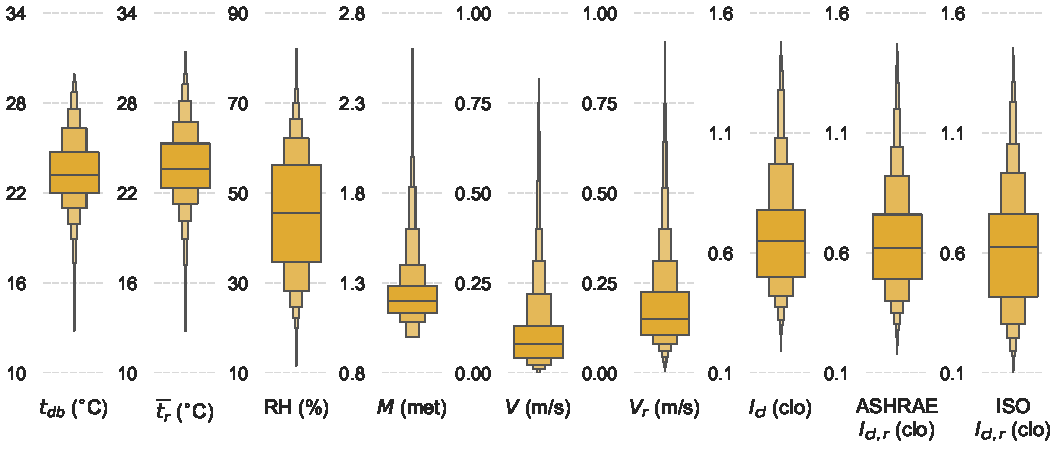
\includegraphics[width=\textwidth]{figures/dist_input_data}
    \caption{Distribution of the input variables used to calculate the \ac{pmv} and \ac{pmv-ce} values.
    The data are shown using boxen plots (letter-value plots).
    They depict the median as the center-line and each successive level outward contains half of the remaining data.}
    \label{fig:dist_input_data}
\end{figure*}
The input data distributions are far from uniformity (equal density) across the standards' applicability ranges.
We were not able to determine the accuracy of the \ac{pmv} and \ac{pmv-ce} formulations for inputs that are lower than the 2.5th and 97.5th percentiles, since we only had a limited number of data points beyond those values.
For example, only \qty{2.5}{\percent} of the available dataset had a \ac{tdb}~$\leq$ than \var{ta_95_perc_min}, this is a problem since both thermal comfort standards' applicability limits extend to \qty{10}{\celsius}.
This can be explained by the fact that only a few buildings in the world operate at \ac{tdb} lower than this value.
Mainly because an indoor \ac{tdb} lower than \var{ta_95_perc_min} would be deemed to be unsatisfactory by a great number of occupants~\cite{iso7730}.
This lack of data in the \ac{db2} is particularly relevant for \ac{v}.
The \ac{pmv} and \ac{pmv-ce} only differ when the value of \ac{v}~$\geq$~\qty{0.1}{\m\per\s}.
The median value in the \ac{db2} is \var{v_median} suggesting that most of the data points were collected in buildings with low air movement.
We also could not reliably test the accuracy of the \ac{pmv} formulations for values of \ac{v}~$\geq$~\var{v_95_perc_max}.

Figure~\ref{fig:dist_other_data} shows the distribution of age, height, weight, and running mean outdoor temperature.
\begin{figure*}[htb!]
    \centering
    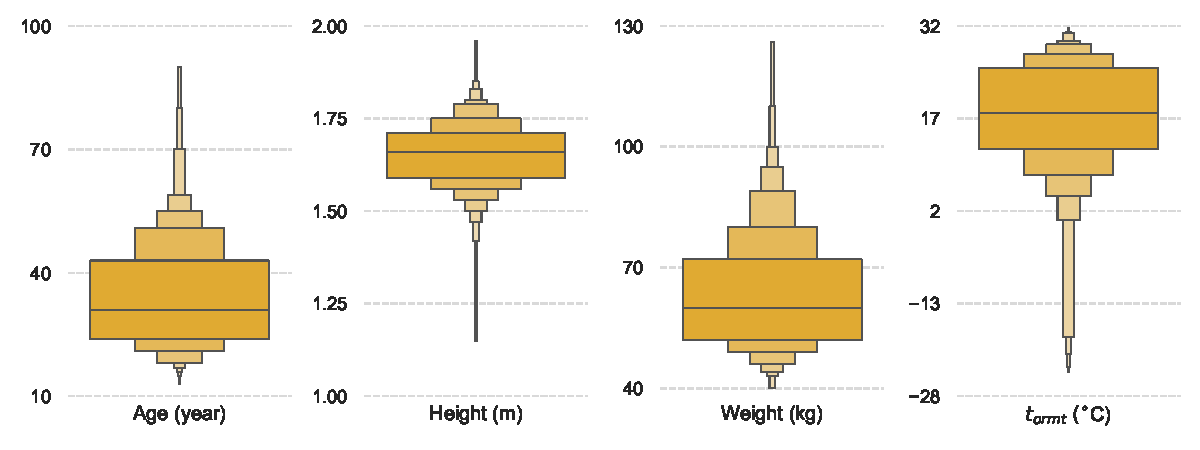
\includegraphics[width=\textwidth]{figures/dist_other_data}
    \caption{Distribution of age, height, weight, and running mean outdoor temperature.}
    \label{fig:dist_other_data}
\end{figure*}
Less than half (\var{entries_with_sex_info}) of the total entries have information about the participant's sex, and are almost equally distributed among males (\qty{52}{\percent}) and females.
Ages are not normally distributed, the same is true for the running mean outdoor temperature.
About half of the participants (\var{percentage_age_20_35}) were aged between \num{20} and \num{35} years old, and only \var{percentage_age_over_60} were older than 60.
This limits our analysis to young adults and does not allow us to determine the accuracy of the \ac{pmv} and \ac{pmv-ce} models in predicting thermal sensation for children or older adults.
The \ac{db2} does not contain information about the health status of the participants.
Approximately \var{running_mean_10_25} of the running mean outdoor temperature values are between \qtyrange{10}{25}{\celsius}.

The percentage of \ac{tpv} grouped by each \ac{tsv} is shown in Figure~\ref{fig:bar_plot_tp_by_ts} a).
\begin{figure*}[htb!]
    \centering
    \begin{subfigure}[b]{\textwidth}
        \centering
        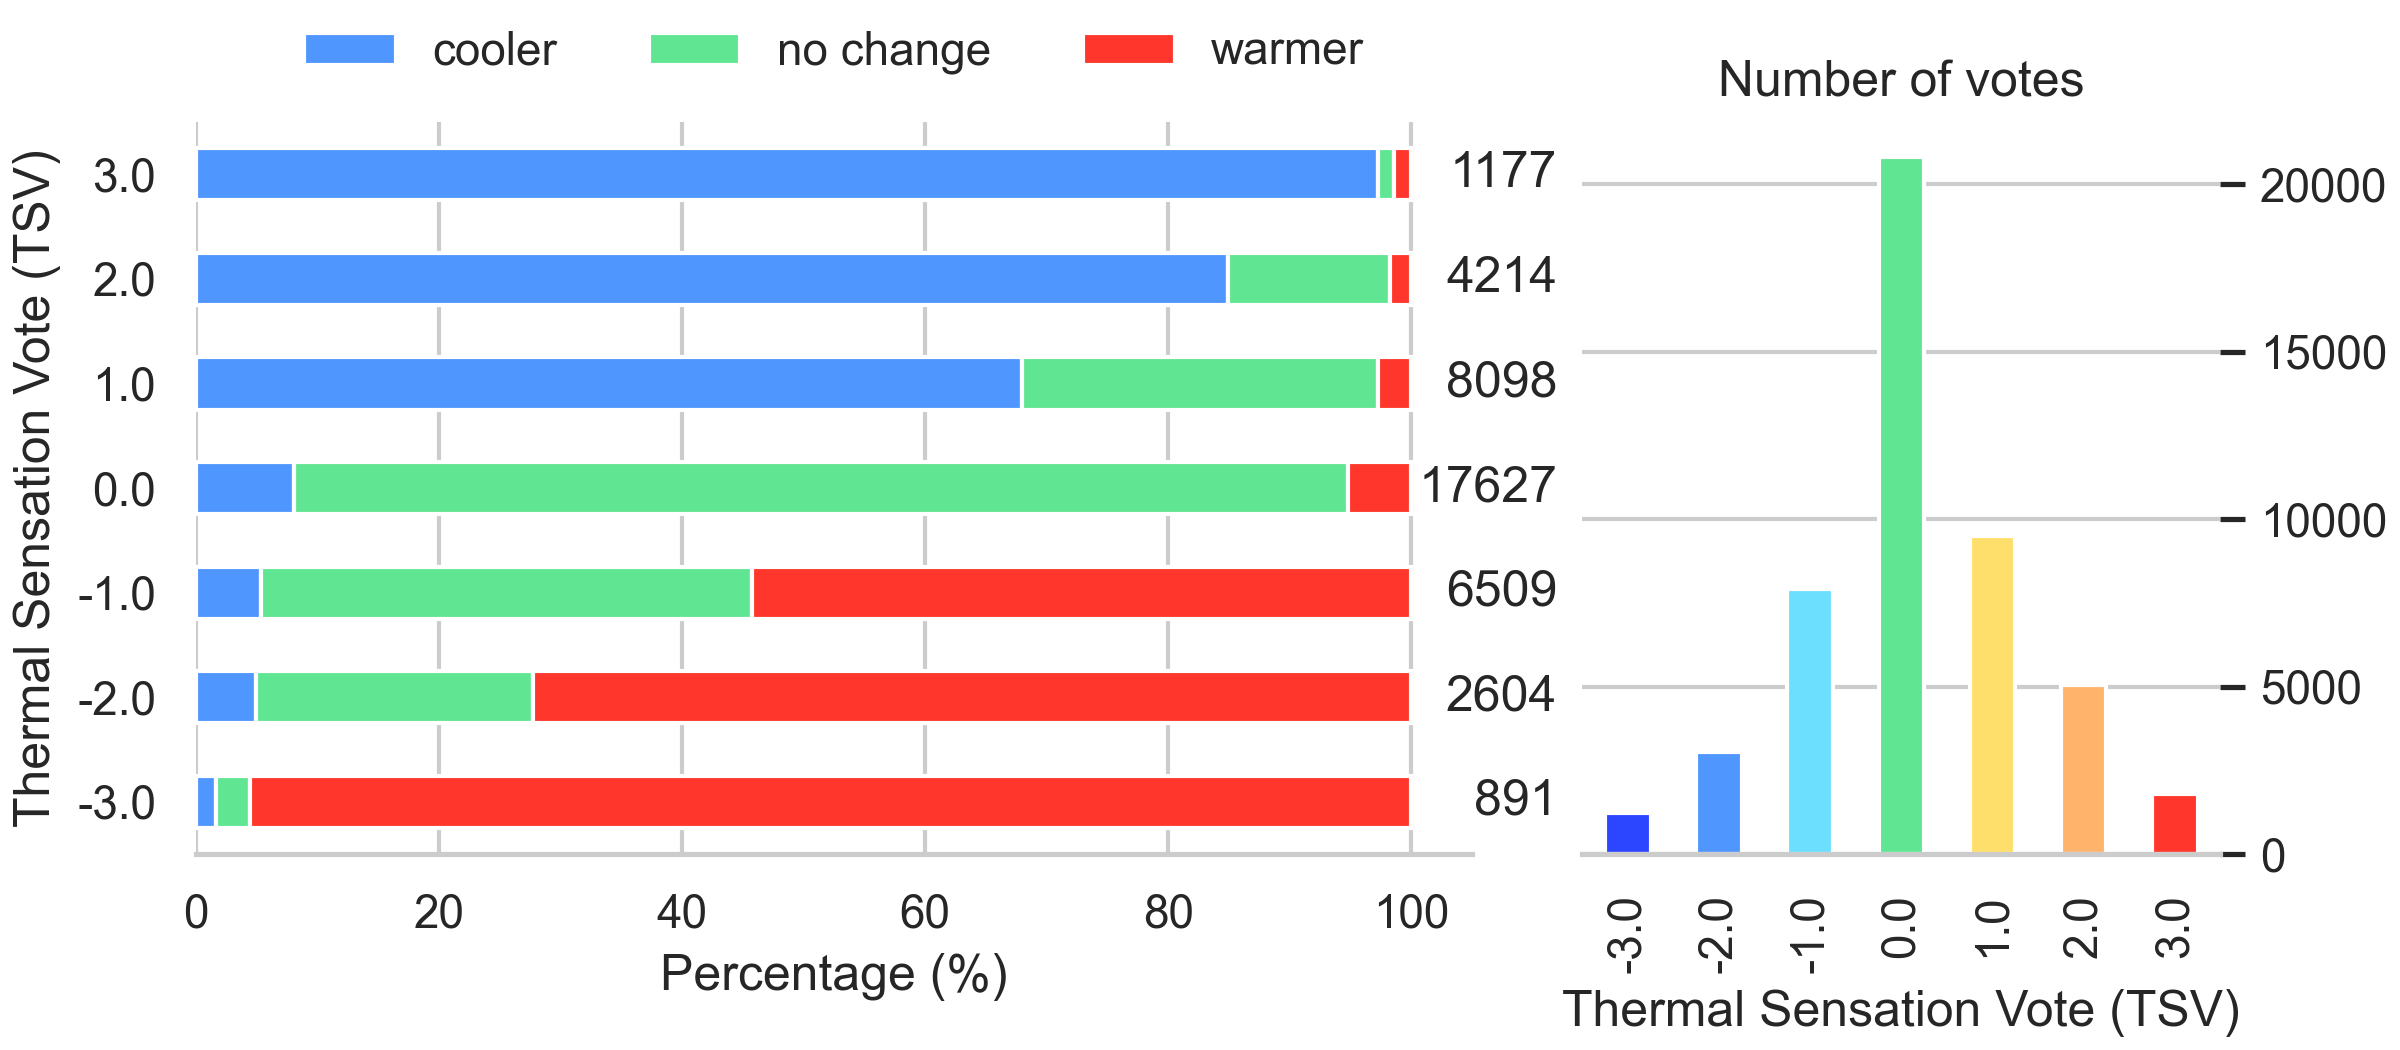
\includegraphics[width=\textwidth]{figures/bar_plot_tp_by_ts}
        \caption{Figure a) shows the percentage of \ac{tpv} for each \ac{tsv}.
    The numbers on the right side of each bar show the number of points for each \ac{tsv}.
        Figure b) shows the total number of data points grouped by \ac{tsv}.
    Each bin in the right figure has more data points than in the left figure, since less data on \ac{tpv} were available.}
    \label{fig:bar_plot_tp_by_ts}
    \end{subfigure}
    \par\bigskip % force a bit of vertical whitespace
    \begin{subfigure}[b]{\textwidth}
        \centering
        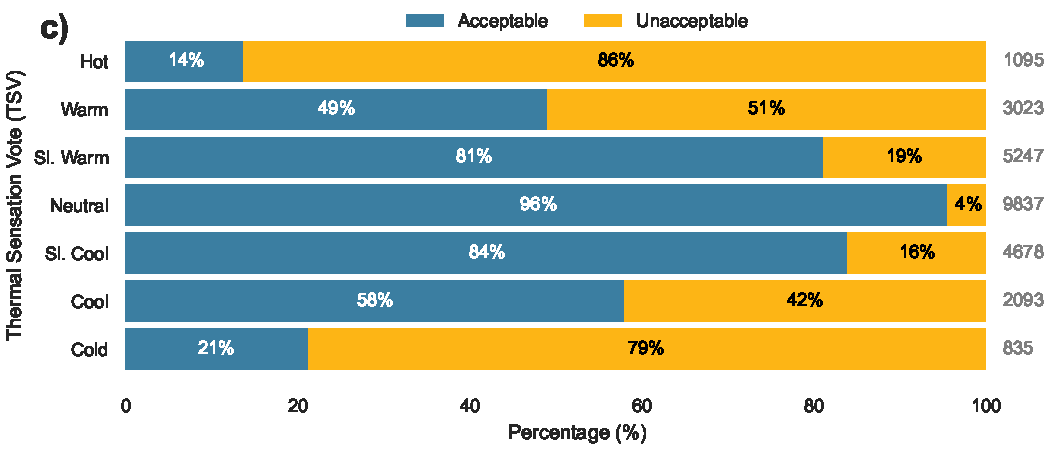
\includegraphics[width=\textwidth]{figures/bar_plot_thermal_acceptability_by_thermal_sensation_round}
    \caption{
        Figure c) shows the percentage of participants who consider the space thermally acceptable for each \ac{tsv}.}
        \label{fig:thermal_acceptability_by_ts}
    \end{subfigure}
    \caption{The distribution of \ac{tpv} and thermal acceptability grouped by each \ac{tsv}.}
\end{figure*}
Only \var{entries_with_tp} entries have information about both \ac{tsv} and \ac{tpv}.
Thus, on the right, we show a bar chart depicting the distribution of all the \ac{tsv} votes, we analyzed in the paper.
The \ac{tsv} dataset is unbalanced.
Approximately \var{perc_tsv_neutral} of all the entries have a \ac{tsv} of `neutral'.
While less than \var{perc_tsv_hot} of the total sample of participants reported to be either `hot' or `cold'.
In thermal comfort research, it is generally assumed that people who are `slightly warm' or `slightly cool' are thermally comfortable~\cite{Fanger1970, schweiker2020evaluating}.
Fanger, in his seminal book on thermal comfort wrote that ``The dissatisfied are defined here as those who vote \num{-2} (cool) or \num{-3} (cold), \num{2} (warm) or \num{3} (hot).
One could perhaps object that those voting \num{-1} or \num{1} were not included also, but as evidenced by Gagge et al., real discomfort is first expressed by those voting higher than \num{2} or lower than \num{-2}.''~\cite{Fanger1970}.
However, \qty{68}{\percent} of participants who were `slightly warm' wanted to be `cooler' and \qty{54}{\percent} of participants who were `slightly cool' wanted to be `warmer'.
This finding challenges the above assumption.
Assuming that people who are `slightly warm' or `slightly cool' are comfortable leads to under-counting thermal discomfort.
On the other hand, some participants who reported to be `cool', `cold', `warm', or `hot' wanted `no change'.
Of those who reported being `cool', \qty{23}{\percent} of them wanted `no change' and \qty{5}{\percent} wanted to be `cooler'.
Similarly, but in reverse, among those who reported being `warm' \qty{13}{\percent} wanted `no change' and \qty{2}{\percent} wanted to be `warmer'.
This result highlights one of the major limitations of the \ac{tsv} scale.
The thermal preference scale is better suited to determine how people perceive their thermal environment and more clearly provides a signal to decide whether to change or not the thermal environment.
On the contrary, the \ac{tsv} is ambiguous and does not allow determining if an action should be taken to increase the participant's thermal comfort.
As illustrated in Figure~\ref{fig:thermal_acceptability_by_ts}, over \qty{80}{\percent} of occupants who feel `slightly warm' or `slightly cool' consider the space thermally acceptable.
However, thermal comfort is defined as ``the state of mind that expresses satisfaction with the thermal environment,'' rather than simply finding the space acceptable. 
This distinction highlights that while many may tolerate slight deviations from their preferred temperature, true thermal comfort involves a higher level of satisfaction with the surrounding thermal conditions.
We did not analyze the thermal comfort data since in the \ac{db2} it is unclear which scale was used to collect the data.

\subsection{Comparison of PMV Accuracy in Predicting Thermal Sensation}\label{subsec:model-accuracy-comparison-in-predicting-thermal-sensation}
The \ac{pmv} was developed with the primary aim of predicting \ac{tsv}, consequently, we compared the predicted value from the two models with measured \ac{tsv}.
However, since the two models only differ when \ac{v}~$>$~\qty{0.1}{\m\per\s};
we also present the results for a subset of the data where \ac{v}~$\geq$~\qty{0.2}{\m\per\s}.
In this subset of data, the differences in the outputs of the two models are more pronounced.
We set the limit to \qty{0.2}{\m\per\s} and not a higher value since, as previously shown in Figure~\ref{fig:dist_input_data}, we could only reliably test the accuracy of the models up to \ac{v} of \var{v_95_perc_max}.

Being \ac{tsv} the value reported by participants (i.e., ground truth), in Figure~\ref{fig:bar_stacked_model_accuracy} we grouped participants' responses by \ac{tsv} and reported the simple accuracy of the different \ac{pmv} formulations over each sub-figure.
\begin{figure}[htb!]
    \centering
    \begin{subfigure}[b]{\textwidth}
        \centering
        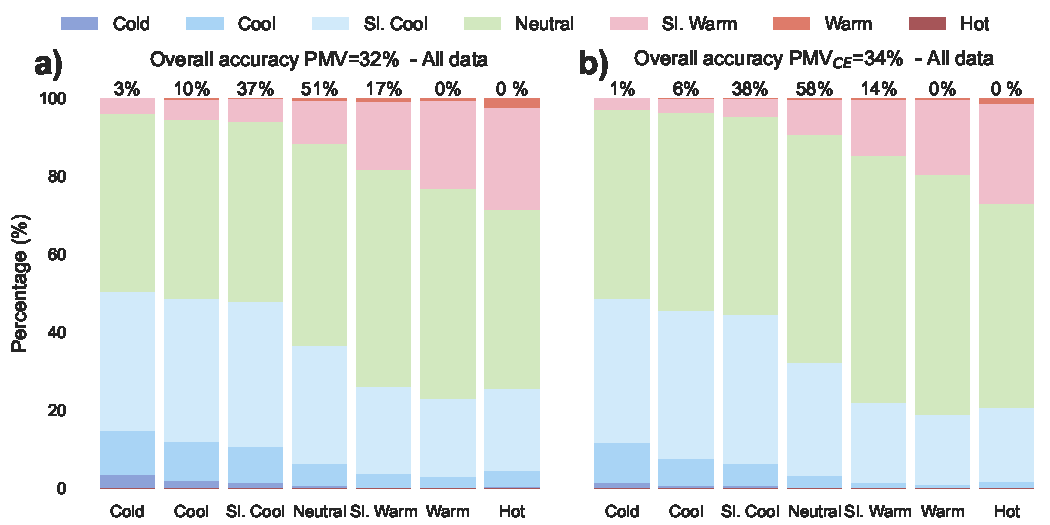
\includegraphics[width=\textwidth]{figures/bar_stacked_model_accuracy_0}
    \end{subfigure}
    \par\bigskip % force a bit of vertical whitespace
    \begin{subfigure}[b]{\textwidth}
        \centering
        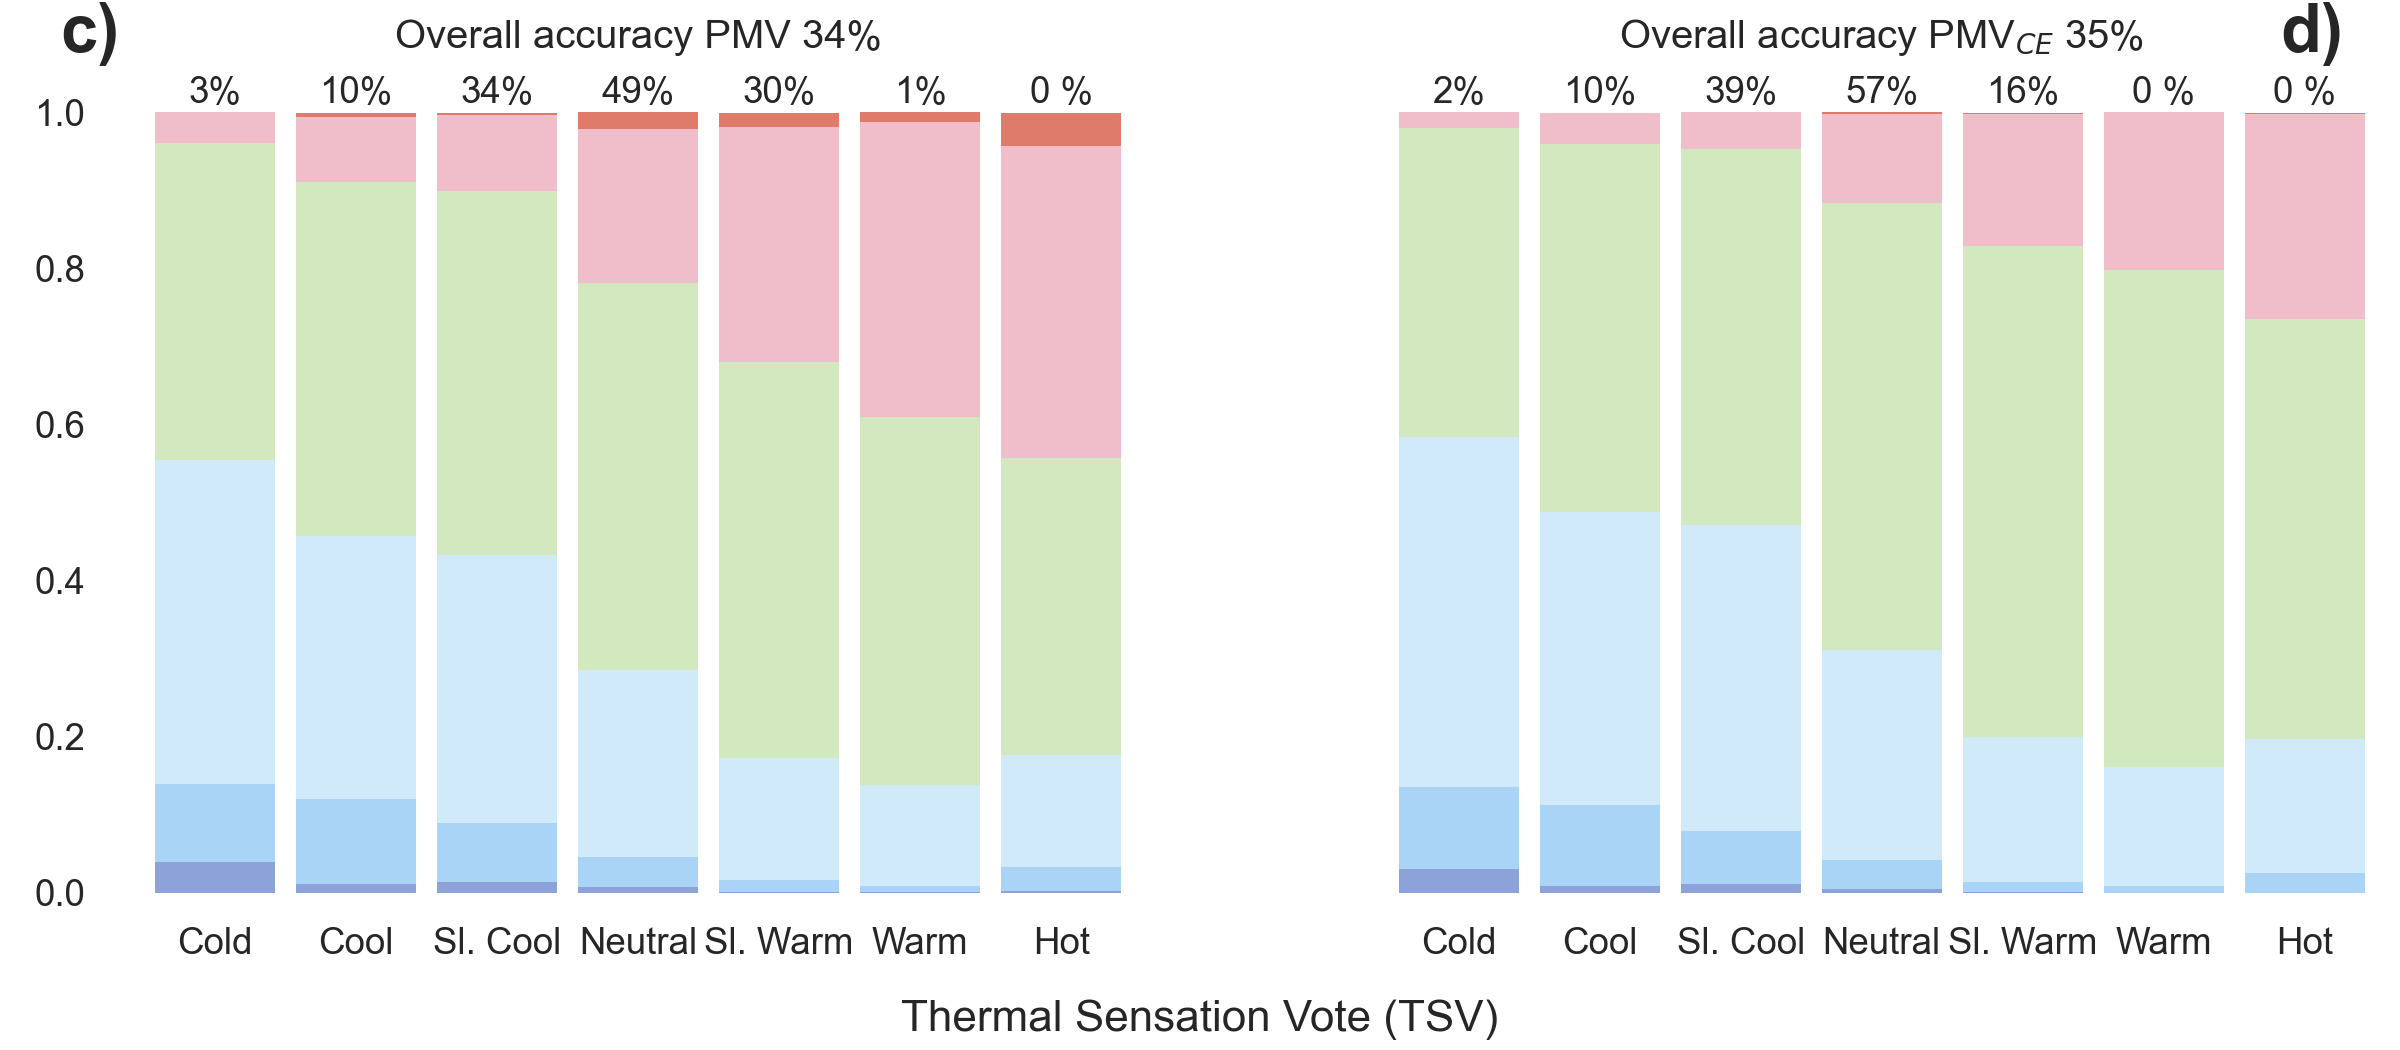
\includegraphics[width=\textwidth]{figures/bar_stacked_model_accuracy_0.2}
    \end{subfigure}
    \caption{The calculated \ac{pmv} value is grouped by the \ac{tsv} value reported by the participants.
    In a) and b) for the entire dataset, while in c and d for the dataset when \ac{v}~$\geq$~\qty{0.2}{\m\per\s}.
    In a) and c) are shown the results for the \ac{pmv} model, and in b) and d) for the \ac{pmv-ce} model.
    The number of data points in each bin of the two charts at the top (a and b) and at the bottom (c and d) is the same, and this allows us to compare the accuracy of both models.
    The overall prediction accuracy is shown above the chart, while the model accuracy of predicting participants grouped by their \ac{tsv} is shown over each bar.
    A random model would have an accuracy of \qty{14}{\percent}.}
    \label{fig:bar_stacked_model_accuracy}
\end{figure}
Both \ac{pmv} formulations underestimate the conditions at which participants are thermally dissatisfied with their environment.
The overall accuracies of the \ac{pmv} and \ac{pmv-ce} are \qty{33}{\percent} and \qty{34}{\percent}, respectively, when using the whole dataset.
The overall accuracy of both \ac{pmv} models increase to \qty{34}{\percent} and \qty{35}{\percent}, respectively when only considering entries with \ac{v}~$\geq$~\qty{0.2}{\m\per\s}.
The \ac{pmv-ce} model outperforms the \ac{pmv} model for \ac{tsv}~=~0 and -1.
However, the \ac{pmv} model outperforms the \ac{pmv-ce} model when considering \ac{tsv}~=~1.
The number of data points in each \ac{tsv} bin is different.
\mycite{Cheung2019} grouped people based on the same heat loss or gains (same \ac{pmv} ranges), not the same \ac{tsv} as we did here, and then quantified the sensitivity of the model, i.e., how many times the \ac{pmv} model correctly predicted \ac{tsv}.
They found that the accuracy of \ac{pmv} in predicting \ac{tsv} was only \qty{34}{\percent} \mycite{Cheung2019}.

Being the classification problem unbalanced, the simple accuracy is not an optimal metric to rate the model prediction accuracy, since a default strategy of guessing the majority class would lead to a high overall model accuracy.
A model that always predicts `neutral' would achieve an overall accuracy of \var{perc_tsv_neutral}, the number of participants who voted \ac{tsv}~=~0.

In Table~\ref{tab:f1}, we report the F1 scores for both models, i) using the whole dataset, ii) only keeping entries with \ac{v}~$\geq$~\qty{0.2}{\m\per\s}, iii) only keeping data points that have \ac{v} measured at three heights with \ac{v}~$\geq$~\qty{0.2}{\m\per\s}, and iv) for those with a $\lvert \textrm{PMV}\lvert \leq 1.5$ and $\lvert \textrm{TSV}\lvert \leq 1.5$.
\begin{table}[htb!]
    \centering
    \begin{tabular}{lccc}
\toprule
F1 score & PMV & PMV$_{CE}$ & Dataset \\
\midrule
 micro & 0.32 & 0.34 & \multirow{3}{*}{All data} \\
macro & 0.16 & 0.15 &  \\
weighted & 0.29 & 0.30 &  \\
\specialrule{.01em}{.05em}{.05em} micro & 0.32 & 0.35 & \multirow{3}{*}{\ac{vr} $\geq$ \qty{0.2}{\m\per\s}} \\
macro & 0.17 & 0.17 &  \\
weighted & 0.30 & 0.31 &  \\
\specialrule{.01em}{.05em}{.05em} micro & 0.30 & 0.31 & \multirow{3}{*}{\ac{vr} $\geq$ \qty{0.2}{\m\per\s} at three heights} \\
macro & 0.17 & 0.16 &  \\
weighted & 0.27 & 0.27 &  \\
\specialrule{.01em}{.05em}{.05em} micro & 0.43 & 0.45 & \multirow{3}{*}{$\lvert \textrm{PMV}\lvert \leq 1.5$ and $\lvert \textrm{TSV}\lvert \leq 1.5$} \\
macro & 0.23 & 0.22 &  \\
weighted & 0.42 & 0.43 &  \\
\bottomrule
\end{tabular}

    \caption{F1 scores for the \ac{pmv} and \ac{pmv-ce} models for different subsets of data.}
    \label{tab:f1}
\end{table}
The F1-macro score, which is free from label imbalance, depicts that the accuracy of both models across all metrics is marginally better than random guessing (i.e., \qty{14}{\percent}) for all data.
For the subset of data with \ac{v}~$\geq$~\qty{0.2}{\m\per\s} the F1-macro scores of the \ac{pmv} and \ac{pmv-ce} models only slightly improved.
We then analyzed the subset of data with \ac{v}~$\geq$~\qty{0.2}{\m\per\s} and with \ac{v} measured at three heights.
Both F1-macro scores decrease and the \ac{pmv-ce} (\num{0.16}) is lower than the value for the \ac{pmv}~ (\num{0.17}).
Our results show that the assumption that the \ac{pmv-ce} better takes into account the effect of elevated air speed is false.
All the F1 scores significantly increase when analyzing the dataset with $\lvert \textrm{PMV}\lvert \leq 1.5$ and $\lvert \textrm{TSV}\lvert \leq 1.5$.
This highlights that the \ac{pmv} models are only accurate in predicting the thermal sensation of people when the thermal sensation is close to neutral.

\subsection{Model Bias}\label{subsec:model-bias}
The intended aim of the \ac{pmv} model is not to accurately predict each individual thermal response from participants.
The \ac{pmv} model was developed to predict the average thermal sensation of an undefined large group of occupants sharing the same environment.
The results presented so far are primarily comparing individual \ac{tsv} to \ac{pmv}.
This type of analysis does not conclusively disprove the inefficacy of the \ac{pmv} models in predicting the average thermal sensation of a large group of occupants.
Moreover, grouping the results into discrete categories introduces rounding errors since some participants reported \ac{tsv} on a continuous scale and the \ac{pmv} value is a continuous variable.
To compensate for this we plotted the \ac{pmv} and \ac{pmv-ce} values as a function of \ac{tsv} in Figure~\ref{fig:bubble_models_vs_tsv} and we plotted a \ac{lowess} curve.
\begin{figure*}[htb!]
    \centering
    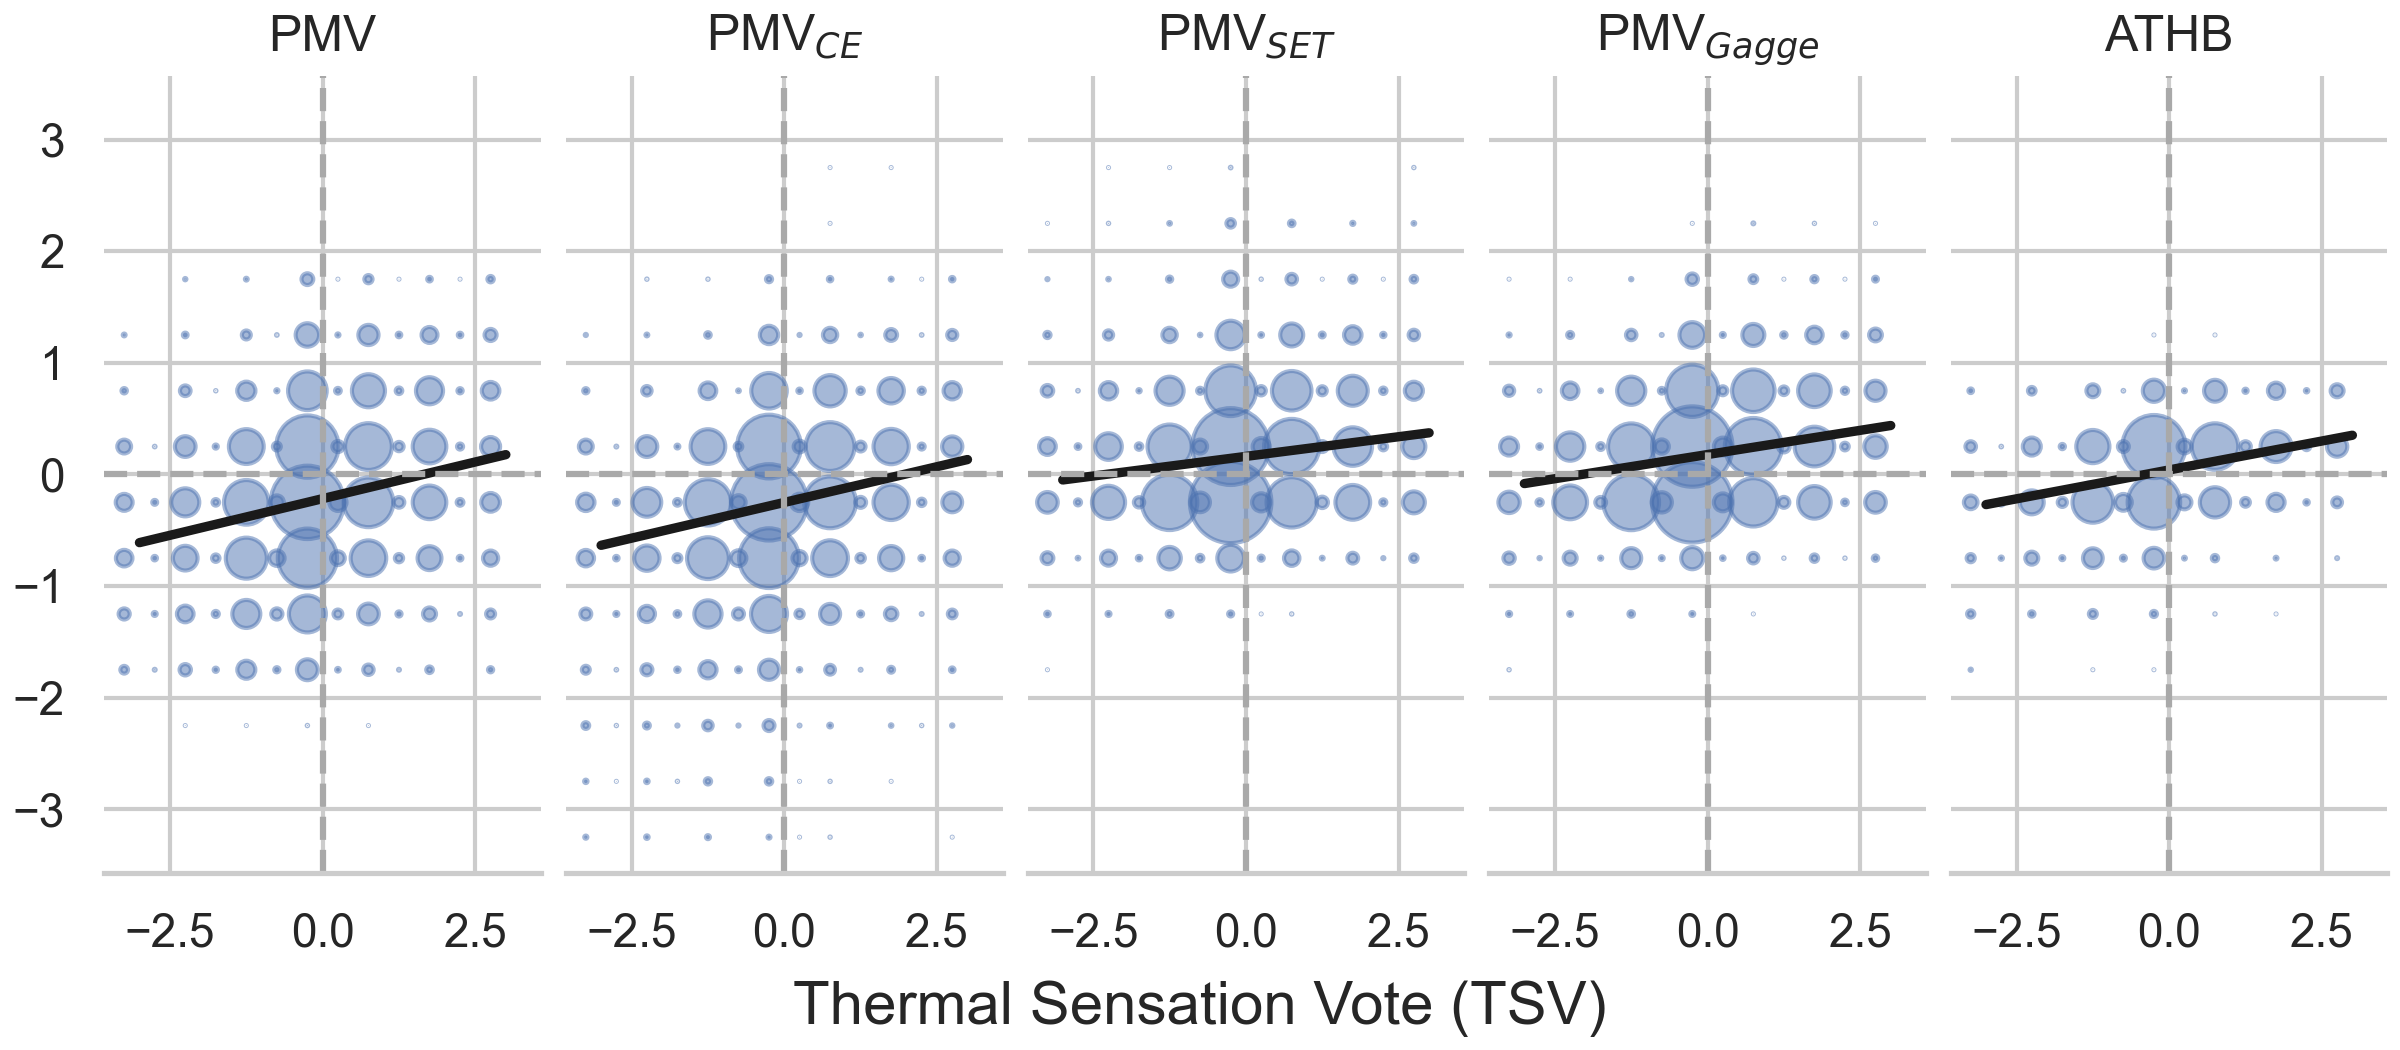
\includegraphics[width=\textwidth]{figures/bubble_models_vs_tsv}
    \caption{The \ac{lowess} curve shows the relationship between the raw \ac{pmv} and \ac{tsv} data.
    Raw data were then binned and a bubble chart (circle area is proportional to the number of votes in that bin) was superimposed over the regression curve to aid the visualization of a large dataset.
    The brown dashed line represents the identity line where the slope is 1 and the intercept is 0.}
    \label{fig:bubble_models_vs_tsv}
\end{figure*}
The curve, in the Figure, is calculated using the individual data and not the binned data.
We only binned the data to aid the visualization of a large dataset.
For the model to accurately predict people’s thermal sensation, the regression line (black continuous line) should pass through the origin of the Cartesian plane and have a slope of 1.
This ideal prediction is referred to as the identity line, shown as the brown dashed line in the figure.
The intercepts for the \ac{pmv} is \qty{-0.22} and for the \ac{pmv-ce} is \qty{-0.24} which means that the model has a bias of less than one-quarter of a thermal sensation interval.
This result is aligned with those presented in Figure~\ref{fig:bar_stacked_model_accuracy} where the \ac{pmv} and \ac{pmv-ce} models can predict people who reported to be neutral \qty{54}{\percent} and \qty{58}{\percent} of the times, respectively.
Both \ac{pmv} formulations always under-predict the thermal sensation of people who reported to be on the extremes of the \ac{tsv};
the slope of the curve was significantly lower than 1.

\subsubsection{Model Overall Bias}\label{subsubsec:model-overall-bias}
We calculated the overall bias of the model as previously done by \mycite{Humphreys2002} by subtracting the \ac{pmv} and \ac{pmv-ce} models prediction from the self-reported \ac{tsv}.
Figure~\ref{fig:hist_discrepancies} contains the summary statistics.
Overall both the \ac{pmv} and \ac{pmv-ce} models have a median bias lower than half of a thermal sensation interval.
The results highlight that the \ac{pmv-ce} has a higher bias than the \ac{pmv} both when calculating the bias for all the data and for the subset of data with \ac{v}~$\geq$~\qty{0.2}{\m\per\s}.
We report the median and inter-quantile ranges since data are not normally distributed.
%  We cannot change into a letter value plot since in that case, it would be hard to highlight the number of responses that are within the range from -.5 to 5.
\begin{figure*}[htb!]
    \centering
    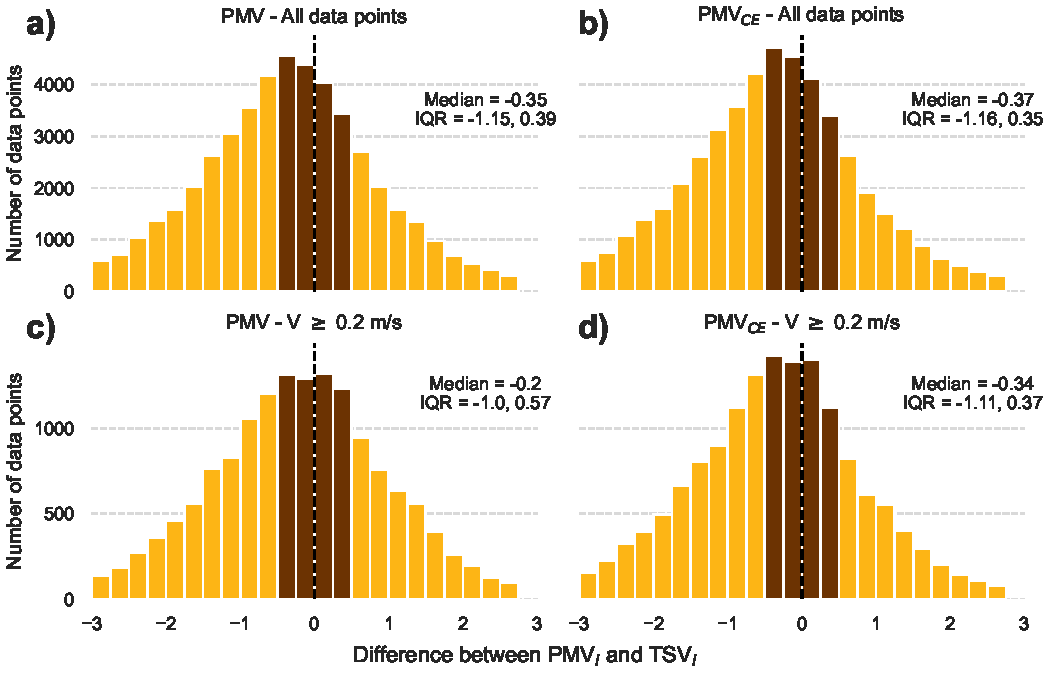
\includegraphics[width=\textwidth]{figures/hist_discrepancies}
    \caption{Overall bias of the \ac{pmv} and \ac{pmv-ce} models for the subset of data with \ac{v}~$\geq$~\qty{0.2}{\m\per\s}.
    The x-axis shows the discrepancy (bias) between the predicted and self-reported \ac{tsv}.
    We have binned the data into intervals of equal width.
    We colored the bars in the range from \num{-.5} to \num{.5} to highlight the number of responses that are within this range.
    The chart also shows the median and inter-quantile ranges of the data.
    }
    \label{fig:hist_discrepancies}
\end{figure*}
When including only the data with \ac{v}~$\geq$~\qty{0.2}{\m\per\s} the median bias of the \ac{pmv} model reduces to \var{bias_median_pmv_0.2} from \var{bias_median_pmv_0}, meaning that at higher speed the \ac{pmv} model improves.
The median bias for the \ac{pmv-ce} also decreases to \var{bias_median_pmv_ce_0.2} from \var{bias_median_pmv_ce_0} but it is higher than the one for the \ac{pmv}.

\subsubsection{Model Bias as Function of Five Input Variables}\label{subsubsec:model-bias-variable}
Here we present the model bias as a function of the five input variables \ac{tdb}, \ac{v}, \ac{rh}, \ac{met}, and \ac{clo}.
Results are shown in Figure~\ref{fig:bias_models}.
\begin{figure*}[htb!]
    \centering
    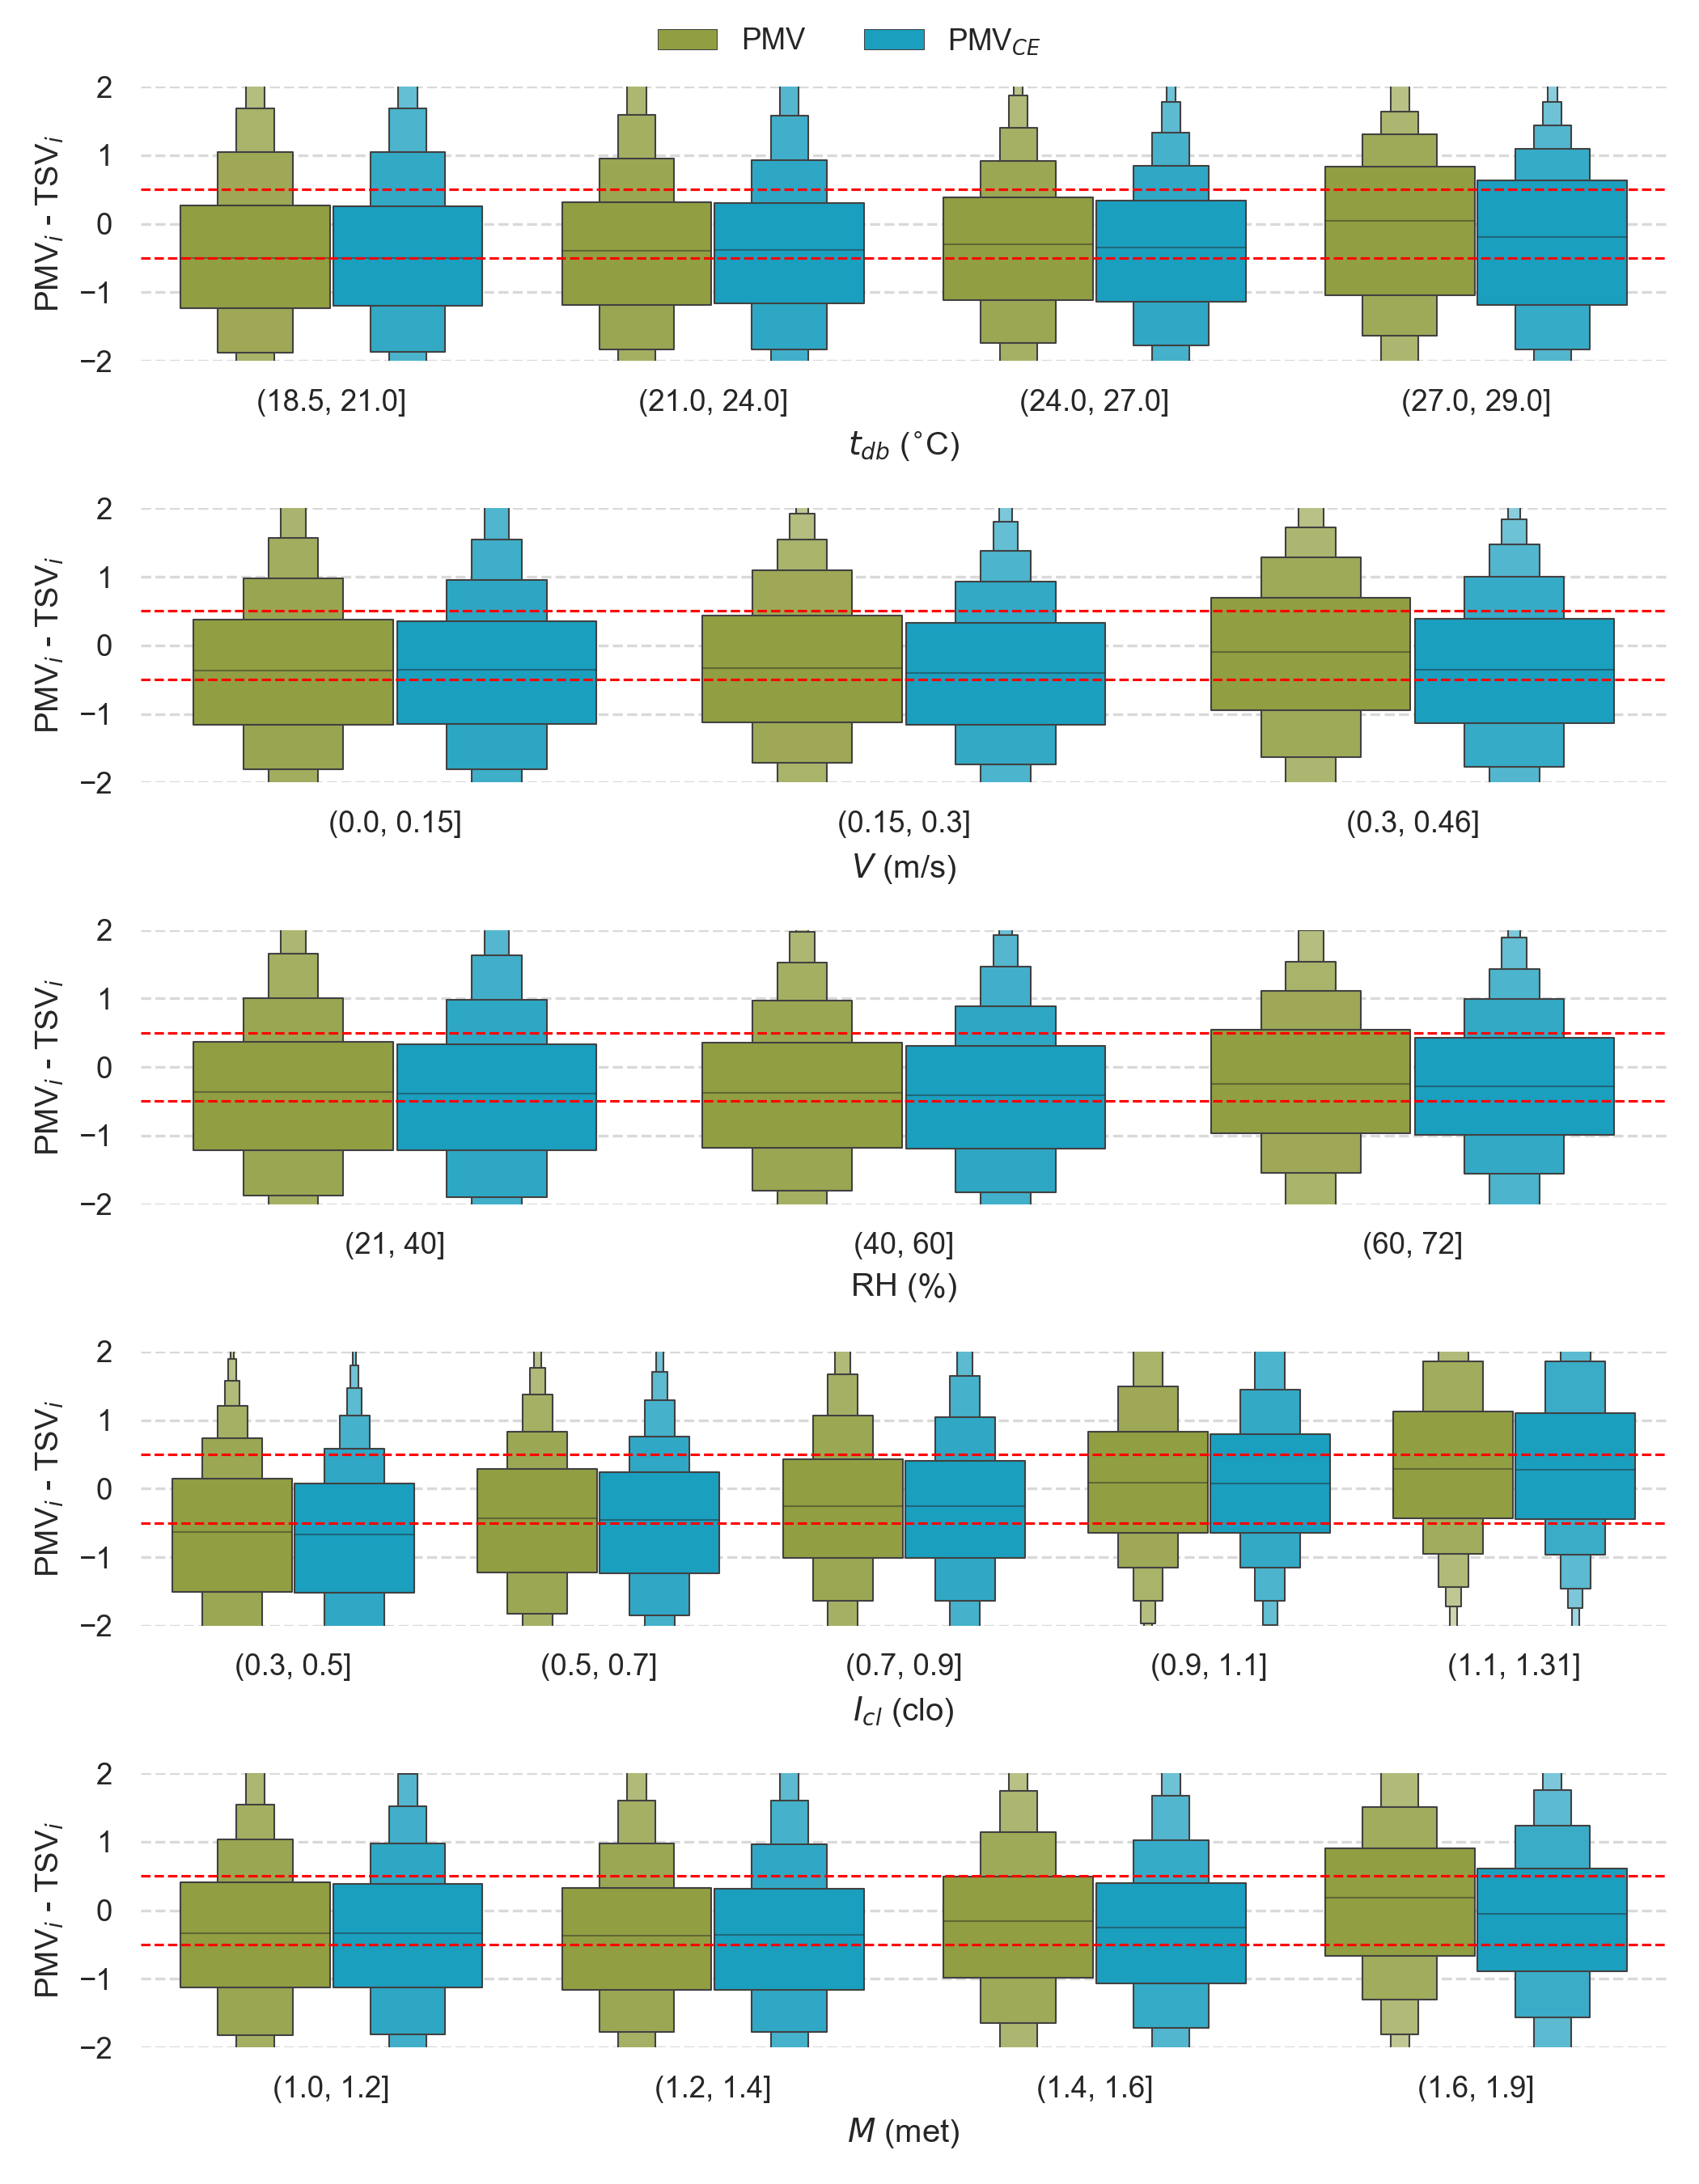
\includegraphics[width=\textwidth]{figures/bias_models}
    \caption{Bias of the \ac{pmv} and \ac{pmv-ce} models plotted as a function of the input variables.
    The x ticks labels show the bin range.
    The square bracket($]$) means that the right value is included in the range.
    The red dashed lines show the acceptable range of bias.
    Each bin has a different number of data points.
    }
    \label{fig:bias_models}
\end{figure*}
In each sub-figure, we have binned the results into discrete intervals.
The x-axis tick label shows the bin range.
All the boxen-plots have the same area to aid visualization, even though the number of points in each bin is not constant.
The results depict that the use of the \ac{pmv-ce} model does not improve the bias of the \ac{pmv} results across all input variables.
On the contrary, the bias of the \ac{pmv-ce} diverges more from 0 and is significantly worse (\num{-.33} versus \num{-0.13}) than the one for the \ac{pmv} for \qty{0.3}{\m\per\s}~$<$~\ac{v}~$\leq$~\qty{0.46}{\m\per\s}.
Both models have a median bias higher or equal to $\lvert0.5\lvert$ for \ac{tdb}~$\leq$~\qty{21}{\celsius} and \ac{clo}~$\leq$~\qty{.5}{clo}.

These findings, along with those shown in Table~\ref{tab:f1} and earlier figures, demonstrate that the \ac{pmv-ce} model has lower accuracy and higher bias compared to the \ac{pmv} at elevated air speeds, even though the \ac{pmv-ce} model is more complex and requires more computational resources.

\subsection{Sources of Error}\label{subsec:sources-of-error}
In this section, we try to identify some of the main reasons that could explain the difference in the results from the two \ac{pmv} models when compared against the \ac{tsv} available in the \ac{db2}.
Moreover, we tried to explain why we observed that the \ac{pmv-ce} model has a lower accuracy than the \ac{pmv} in predicting thermal sensation.
The issues are reported in order of importance of what we believe may affect the accuracy of the model.
\todo{Note that the section below does not mention the two-node model, the CE implementation of PMV, or the physiological differences between the ISO and ASHRAE models that could explain the observed differences or ‘error’. }

\paragraph{Heat Balance Equation and Calculation of the PMV Value}
The \ac{pmv} model uses simplified heat balance equations to estimate the heat losses and gains from the human body to its surrounding environment.
This is a possible source of error since the model considers the human body to be a cylinder with constant width all uniformly covered with clothing where the heat is all generated in its core.
This is a significant simplification, as it overlooks several important factors, such as the uneven coverage of clothing across different parts of the body, the non-uniformity of metabolic heat generation, and the variations of mass-to-surface ratios.
It also ignores vasoconstriction and vasodilation.
Additionally, the \ac{pmv} model erroneously assumes that the human body is not capable of maintaining a stable core temperature.
A \ac{pmv} value higher than \num{.5} or lower than \num{-.5} indicate that the hypothetical cylinder is either gaining or losing heat and consequently it is getting warmer or colder, respectively.
Moreover, the \ac{pmv} model has been developed based on the assumption of steady-state heat transfer; however, this never precisely occurs.
The human thermoregulatory system, in healthy humans, is constantly actively engaged to ensure a stable core temperature~\cite{romanovsky_thermoregulation_2018}.
The \ac{pmv} model also assumes that the human body is constantly losing a certain amount of heat through sweating and this heat loss (W/m\textsuperscript{2}) only varies as a function of \ac{met} and it is calculated using the following equation $0.42\times($\ac{met}$\times58.15 - 58.15)$~\cite{Fanger1970}.
This amount of heat loss is included in the equation even if the cylinder has a negative heat gain, or in other words, the person is estimated to be feeling cold.

The \ac{pmv} model uses the overall heat losses or gains to calculate a \ac{pmv} value which should represent the average \ac{tsv} of a large group of occupants.
Heat losses or gains are only a proxy for the thermoregulation effort that the human body has to undergo to maintain a constant internal temperature.
Fanger created this equation based on a limited dataset collected in a laboratory, and this equation was never updated or revisited~\cite{Fanger1970}.
In the \ac{pmv} model the heat losses and gains are mapped using constant coefficients to a \ac{tsv}, disregarding the fact that the human body employs different strategies, i.e., vasodilation and vasoconstriction to cope with warm and cold conditions~\cite{romanovsky_thermoregulation_2018}.

It is, therefore, not surprising to observe that the \ac{pmv} model has an `acceptable' accuracy only in determining when people are `neutral'.
This is equivalent to no heat losses or gains (i.e., \ac{pmv}=0) which means that the body is dissipating all the internal metabolic heat production through conduction, convection, or radiation without needing to thermoregulate using sweating, shivering, vasoconstriction, vasodilation, behavioral adjustments, and non-shivering thermogenesis~\cite{ romanovsky_thermoregulation_2018}.
On the other hand, the model cannot correctly predict the thermal sensation of people who report being outside the thermal neutrality zone.
The model's inability to account for these regulatory mechanisms is a fundamental limitation.

To continue using the \ac{pmv} model beyond an absolute value of \num{0.5}, more research is needed to determine whether the inaccuracy of the model is related to either or a combination of the following factors and if those sources of inaccuracy can be reduced:
\begin{enumerate}
    \item verify the assumption that the heat losses/gains estimated by the \ac{pmv} are correlated to the thermoregulatory response that the body has to undertake to compensate for unsatisfactory thermal comfort conditions;
    \item if the previous assumption holds, research is needed to validate the correlation coefficients used by Fanger to map the heat losses/gains and thermal stress;
    \item currently a single correlation coefficient is used for the hot and cold side but this may not be a valid assumption and two different sets of equations may be used;
    \item the anchors used by the \ac{pmv} model are different from those used by participants in reporting their thermal sensation.
    The \ac{pmv} model assumes that a score of 3 (`hot') signifies the change between a compensable set of conditions to an un-compensable one, e.g., skin wettedness reaches its max value ($w_{max}$), as suggested by Gagge~\cite{GaggeSET}.
    On the contrary, participants indoors may deem the environment to be `hot' as soon as their \ac{w} crosses a critical threshold, which is only a fraction of $w_{max}$.
\end{enumerate}

A combination of all the above-mentioned factors likely plays a role in explaining the discrepancies between the \ac{pmv} model and the self-reported \ac{tsv}.
The latter hypothesis -- 4) anchoring -- has gained significant momentum in the literature, which led to the development of several \ac{pmv} formulations that apply correction factors to the final \ac{pmv} result without changing the underlying equations~\cite{Yao2022, Toftum2002}.
Supporting evidence was provided by \mycite{schweiker2020evaluating}, who showed that the distances between the anchors are not constant and a layperson may not perceive the \ac{tsv} scale as researchers believe they do~\cite{schweiker2019scales, schweiker2020evaluating}.

\paragraph{Measurement Errors}
All the data contained in the \ac{db2} have been published in peer-reviewed manuscripts; however, measurement errors are inevitably present in the dataset.
Instrumentation is not always calibrated and the uncertainty of the measurements may be large, the placement of the instrumentation may not be in the participant's proximity, and estimating clothing and metabolic rates from tables is a complex and prone-to-error task.
In an ideal scenario, errors would be randomly distributed and cancel out, not significantly affecting the overall bias of the model but only affecting the standard deviation of the error~\cite{Humphreys2002}.
However, this may not always be the case, for example, if a researcher often underestimates participants' clothing insulation or activity levels.
Moreover, most of the data in the \ac{db2} also only contains entries where the air speed was measured at a single height.
This is a problem since the \ac{pmv} model assumes that the air speed is uniform across the human body, and this is not always the case.
Measuring the air speed at a single height may lead to record higher values than the averaged velocities that are required for the standards’ comfort models.
This is because the anemometer is almost always placed in relatively open space between mid-body and head level, avoiding measuring the usually sheltered lower body level, consequently the associated sensation prediction will be cooler than it should be.
To account for this error, we only included the studies where the air speed was measured at three different heights in \ref{sec:analysis-of-the-dataset-with-air-speed-measurements-at-three-heights}.
However, these results were not significantly different from those presented in this paper, and the \ac{pmv-ce} model still had a higher bias than the \ac{pmv} model.

\paragraph{Thermal Sensation Scale}
One minor, but not negligible, source of error is using a discrete scale to assess thermal sensation (most of the \ac{tsv} in the \ac{db2} were collected using a discrete scale) while the \ac{pmv} output is continuous.
For example, even if the model is \qty{100}{\percent} accurate and the estimated \ac{pmv} value is \num{2.5} the person can only report being `warm (\num{2})' or `hot (\num{3})'.
Using a continuous scale, may in principle be a more robust approach since the distances between the anchors are not constant~\cite{schweiker2019scales, schweiker2020evaluating}.
They also showed that the \ac{tsv} assumption of its independence from contextual factors such as climate, season and language is flawed~\cite{schweiker2019scales, schweiker2020evaluating}.
An alternative solution would be to transform the \ac{pmv} output to an ordinal seven-point scale.